\section{AuthGuard-7702 System Design}
\label{sec:design}

\subsection{Screening workflow}

AuthGuard-7702 is an evaluation-grade scorer positioned inside, but not equal to, a pre-authorization wallet workflow. An external integration parses an authorization request, obtains the runtime bytecode of the named delegate, and supplies that bytecode to AuthGuard. For input bytecode $b$, the implemented path computes the deterministic representation $\phi(b)$ and the classifier score
\begin{equation}
  s=f_{\theta}(\phi(b))\in[0,1],\qquad
  \hat{y}=\mathbb{1}[s\geq\tau].
\end{equation}
Here, $\theta$ is a fitted model and $\tau$ is frozen by the applicable experimental protocol. The score is the model's positive-class output, not a calibrated probability of theft; $\hat{y}$ is a warning signal for the external integration, not an authorization decision.

The interface is intentionally context-free. It accepts a bytecode string rather than an address, chain, transaction, or signer profile, so identical supplied bytecode deterministically yields the same representation before model scoring. The caller remains responsible for resolving the authorization target and supplying the intended runtime. In particular, AuthGuard does not verify that retrieval succeeded, follow proxy or delegation chains, or predict how storage state, call data, and counterparties will affect execution. Those omissions define the scorer's input contract as well as its deployment limit.

Figure~\ref{fig:system-architecture} separates the implemented scorer from prospective integration. Solid boxes show the online bytecode-to-score path and the offline fitting path. Dashed boxes show the authorization, retrieval/cache, and warning components that a wallet or service would need but that we did not implement or evaluate. The offline path produces the model and threshold consumed by online scoring.

% Requires \usepackage{tikz}. No TikZ libraries are required.
\begin{figure}[t]
  \centering
  \resizebox{\columnwidth}{!}{%
  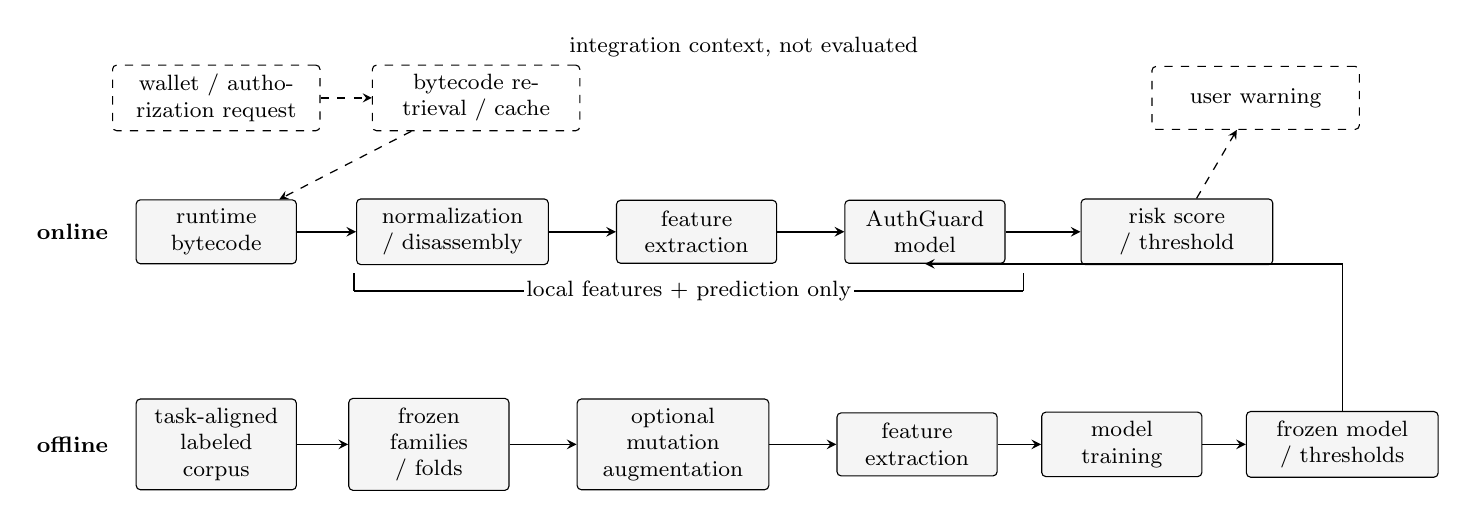
\begin{tikzpicture}[
      font=\footnotesize,
      box/.style={draw=black, rounded corners=1.5pt, minimum height=8mm,
                  text width=22mm, align=center, fill=gray!8},
      smallbox/.style={draw=black, rounded corners=1.5pt, minimum height=8mm,
                       text width=18mm, align=center, fill=gray!8},
      ext/.style={draw=black, dashed, rounded corners=1.5pt, minimum height=8mm,
                  text width=24mm, align=center, fill=white},
      flow/.style={draw=black, ->, >=stealth, line width=.55pt},
      context/.style={draw=black, dashed, ->, >=stealth, line width=.45pt}
    ]
    % External integration context.
    \node[ext] (request) at (0,5.6) {wallet / authorization request};
    \node[ext] (retrieve) at (3.3,5.6) {bytecode retrieval / cache};
    \node[ext] (warning) at (13.2,5.6) {user warning};
    \draw[context] (request) -- (retrieve);
    \node[align=center] at (6.7,6.25) {integration context, not evaluated};

    % Implemented online scorer.
    \node[smallbox] (runtime) at (0,3.9) {runtime bytecode};
    \node[box] (norm) at (3.0,3.9) {normalization / disassembly};
    \node[smallbox] (features) at (6.1,3.9) {feature extraction};
    \node[smallbox] (model) at (9.0,3.9) {AuthGuard model};
    \node[box] (decision) at (12.2,3.9) {risk score / threshold};
    \draw[context] (retrieve) -- (runtime);
    \draw[flow] (runtime) -- (norm);
    \draw[flow] (norm) -- (features);
    \draw[flow] (features) -- (model);
    \draw[flow] (model) -- (decision);
    \draw[context] (decision) -- (warning);
    \node[anchor=east] at (-1.25,3.9) {\textbf{online}};

    % Timing boundary (normalization/disassembly is part of feature construction).
    \draw[line width=.5pt] (1.75,3.15) -- (10.25,3.15);
    \draw[line width=.5pt] (1.75,3.15) -- (1.75,3.38);
    \draw[line width=.5pt] (10.25,3.15) -- (10.25,3.38);
    \node[fill=white, inner sep=1pt] at (6.0,3.15)
      {local features + prediction only};

    % Implemented offline fitting path.
    \node[smallbox] (corpus) at (0,1.2) {task-aligned labeled corpus};
    \node[smallbox] (folds) at (2.7,1.2) {frozen families / folds};
    \node[box] (augment) at (5.8,1.2) {optional mutation augmentation};
    \node[smallbox] (offfeat) at (8.9,1.2) {feature extraction};
    \node[smallbox] (training) at (11.5,1.2) {model training};
    \node[box] (frozen) at (14.3,1.2) {frozen model / thresholds};
    \draw[flow] (corpus) -- (folds);
    \draw[flow] (folds) -- (augment);
    \draw[flow] (augment) -- (offfeat);
    \draw[flow] (offfeat) -- (training);
    \draw[flow] (training) -- (frozen);
    \draw[flow] (frozen.north) |- (model.south);
    \node[anchor=east] at (-1.25,1.2) {\textbf{offline}};
  \end{tikzpicture}%
  }
  \caption{AuthGuard-7702 architecture. Solid nodes are implemented scorer and training paths; dashed nodes and arrows are integration context, not evaluated. The timing boundary covers only local feature construction and prediction.}
  \label{fig:system-architecture}
\end{figure}


\subsection{Deterministic bytecode representation}

Normalization lowercases hexadecimal text, removes a leading \texttt{0x}, and drops a trailing odd nibble. A deterministic linear sweep then tokenizes the byte stream. All \texttt{PUSH1}--\texttt{PUSH32} instructions map to one \texttt{PUSH} opcode token while their declared immediate widths remain available to structural features. Known bytes receive canonical opcode names and other bytes receive stable \texttt{UNK\_xx} tokens. Malformed hexadecimal is handled best-effort by filtering nonhexadecimal characters; a truncated push is advanced according to its declared width, and an incomplete four-byte immediate is not recorded as a selector. Thus the implementation remains total on imperfect inputs without asserting that a linear sweep recovers reachable control flow.

The representation has 773 inputs. First, a 225-dimensional opcode histogram records each token's frequency normalized by the number of decoded operations. Second, 36 structural and selector-related features record byte length; opcode and selector counts; whether the input has the 23-byte delegation-designator shape; counts of jumps, jump destinations, call-family operations, creation, self-destruction, storage access, logs, reverts, invalid/unknown operations, and pushes; mean and selected push widths; jump-destination, call, and push densities; sensitive-selector indicators; and indicators for seven generic interfaces (\texttt{transfer}, \texttt{transferFrom}, \texttt{approve}, \texttt{safeTransferFrom}, \texttt{withdraw}, \texttt{owner}, and \texttt{execute}). These form the 261-dimensional dense block. Finally, opcode 4-grams are deterministically mapped with seeded BLAKE2b into 512 bins and normalized by the number of distinct 4-grams. Histogram, structural, and hashed-gram blocks are concatenated without feature fitting.

One feature implementation is shared by bulk corpus extraction, on-the-fly mutant generation, adversarial augmentation, and online timing. This prevents training/test drift caused by separate parsers. The representation is deliberately syntactic: it does not decompile, resolve reachability, follow proxy implementations, or model execution context.

\subsection{Excluded inputs and classifier}

Only runtime-bytecode-derived values enter $\phi(b)$. Source labels, the class field, source capability columns, chain, address, frozen family identifier, fold assignment, and label-derived oracle verdicts are excluded. The source value-receiving-hook and unrestricted-external-call capabilities are especially unsuitable because they participate in the source labeling procedure; class and oracle fields would restate the target, while chain and family can encode provenance or split identity. Excluding them reduces direct label and provenance leakage, but does not establish that every indirect shortcut or label bias has been removed.

The estimator is standard XGBoost with 300 trees, maximum depth 6, learning rate 0.1, row subsampling 0.9, column subsampling 0.8, histogram tree construction, four worker threads, and random seed 7702. The clean model sets neither an explicit class-weight parameter nor nonuniform sample weights. Its \texttt{predict\_proba} positive-class output is $s$. Boosted trees accommodate the mixture of bounded histogram values, sparse hashed counts, and unscaled structural counts, allow nonlinear interactions, and retain a low-cost prediction path. The estimator itself is not a research contribution.

We use \emph{AuthGuard-M0} for this estimator fitted only on original M0 samples. \emph{AuthGuard-aug} has the same features and hyperparameters but is fitted under the frozen source-balanced augmentation protocol in Section~\ref{sec:methodology}; its weighting is not class rebalancing. Protocol-specific thresholds are learned separately and never treated as model calibration.

\subsection{Local processing boundary}

The measured local path begins with runtime bytecode already loaded in memory and includes normalization, disassembly, feature construction, and model prediction. It excludes model loading, authorization parsing, RPC access, network/cache latency, threshold presentation, warning rendering, and wallet integration. Accordingly, we describe the measurement only as local feature extraction plus prediction, not end-to-end wallet latency. AuthGuard currently provides the scoring core and experimental harness; it is not a production parser, fetch service, model-serving API, extension, or user interface.
